\subsection{LGCN PAS and NGCF PAS}\label{subsec:simple-extension}
\begin{figure}
    \centering
    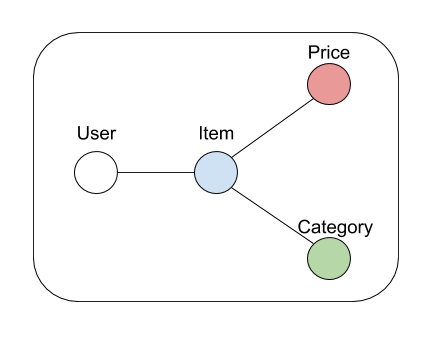
\includegraphics[scale=0.5]{figures/uipc.png}
    \caption{Illustration of the nodes in the simple extension of LightGCN and NGCF.}
    \label{fig:uipc}
\end{figure}
We extend the implementations of LightGCN and NGCF by changing the input parameters, where we construct the adjacency matrix containing the users, item, category and price graph, which is illustrated in \autoref{fig:uipc}.
This extension for LightGCN is called LGCN PAS and the extension of NGCF is called NGCF PAS.
The intuition behind the extension is that the graph convolutions will capture the values of categories and prices, so even if we do not use the embeddings for price and category, they will still influence users and items through the convolutions.
Let the user-item, item-price and item-category interactions matrix be $R \in \mathbb{R}^{I \times U + C + P}$, where $I$ denotes the number of items, $U, C, P$ denotes the number of users, categories and prices.
Each entry of $R_{ui}$ is 1 if user $u$ has rated item $i$. Otherwise it is 0.
If there is a connection in $R_{ic}$ or $R_{ip}$ the value is set to a hyperparameter $x$ defined as:
\[
    x= 
\begin{cases}
    x  & \text{if } x \geq 0\\
    0, & \text{otherwise}
\end{cases}
\]
The adjacency matrix is obtained as follows:
\begin{gather}
    A =
    \begin{bmatrix}
        0   & R \\
        R^T & 0
    \end{bmatrix}
\end{gather}
The embeddings for users and items are calculated for NGCF as described in \autoref{subsubsec:NGCF-embed} and for LightGCN as described in \autoref{subsubsec:lightgcn-embedding}.
The only difference in our implementation is that there are constructed additional embeddings for category and price that are used in the convolutions.
